% =====================================================================
%  PRESENTACION-WIDROW-LEHR.TEX
%  30 Años de Redes Neuronales Adaptativas: Perceptrón, Madaline y
%  Backpropagation (Widrow & Lehr, 1990).
%  Magíster en Ingeniería Informática USACH — Inteligencia Computacional 2026-1.
%
%  Estilo (colores, tema, márgenes, índice, portada) tomado de
%  example-presentation.tex (plantilla USACH).
%
%  Compilación:  pdflatex presentacion-widrow-lehr.tex   (x2)
% =====================================================================

\documentclass[aspectratio=169, 11pt, xcolor={dvipsnames,table}]{beamer}

% ── Paquetes base ────────────────────────────────────────────────────
\usepackage[utf8]{inputenc}
\usepackage[T1]{fontenc}
% Usa 'spanish' si la distribución lo tiene (tu equipo); si no, cae a 'english'
% para poder compilar igual en entornos sin babel-spanish. El contenido no cambia.
\IfFileExists{spanish.ldf}{%
  \usepackage[spanish, es-tabla, es-noshorthands]{babel}%
}{%
  \usepackage[english]{babel}%
}
\IfFileExists{lmodern.sty}{\usepackage{lmodern}\usepackage{microtype}}{}
\usepackage{amsmath, amssymb, mathtools, bm}
\usepackage{graphicx}
\usepackage{booktabs, array, multirow}
\usepackage{multicol}
\usepackage{caption}
\captionsetup{font=footnotesize, labelfont=bf}
\usepackage{tcolorbox}
\tcbuselibrary{skins}
\usepackage{tikz}
\usetikzlibrary{positioning, arrows.meta, calc, shapes.geometric, fit, backgrounds}
\hypersetup{hidelinks}
\usepackage{xcolor}

% ── Paleta USACH ─────────────────────────────────────────────────────
\definecolor{UsachAzul}{RGB}{7,27,73}
\definecolor{UsachNaranja}{RGB}{221,121,0}
\definecolor{UsachGris}{RGB}{57,64,73}
\definecolor{UsachGrisClaro}{RGB}{230,230,230}

% ── Theme + colores Beamer ───────────────────────────────────────────
\usetheme{Madrid}
\useinnertheme{rectangles}
\useoutertheme{infolines}
\setbeamertemplate{headline}{}
\setbeamertemplate{navigation symbols}{}

% - Reducir espacio entre bloques para aprovechar mejor la diapositiva -
\setlength{\medskipamount}{3pt plus 1pt minus 1pt}

% - AUTO-SHRINK MODERADO + MARGEN INFERIOR ---------
\makeatletter
\let\beamer@@frameORIG\beamer@@frame
\def\beamer@@frame[#1]{\beamer@@frameORIG[shrink=55,#1]}
\makeatother

% - FOOTLINE COMPACTA -----------------
\setbeamertemplate{footline}{%
  \leavevmode%
  \hbox{%
  \begin{beamercolorbox}[wd=.32\paperwidth,ht=2.25ex,dp=1ex,center]{author in head/foot}%
    \usebeamerfont{author in head/foot}\insertshortauthor
  \end{beamercolorbox}%
  \begin{beamercolorbox}[wd=.36\paperwidth,ht=2.25ex,dp=1ex,center]{title in head/foot}%
    \usebeamerfont{title in head/foot}\insertshorttitle
  \end{beamercolorbox}%
  \begin{beamercolorbox}[wd=.32\paperwidth,ht=2.25ex,dp=1ex,right]{date in head/foot}%
    \usebeamerfont{date in head/foot}\insertshortdate{}\hspace*{1.2em}%
    \insertframenumber{} / \inserttotalframenumber\hspace*{1.2ex}%
  \end{beamercolorbox}}%
  \vskip0pt%
}

\setbeamercolor{structure}{fg=UsachAzul}
\setbeamercolor{palette primary}{bg=UsachAzul, fg=white}
\setbeamercolor{palette secondary}{bg=UsachAzul!80, fg=white}
\setbeamercolor{palette tertiary}{bg=UsachAzul, fg=white}
\setbeamercolor{title}{fg=UsachAzul, bg=white}
\setbeamercolor{frametitle}{fg=white, bg=UsachAzul}
\setbeamercolor{section in head/foot}{bg=UsachAzul, fg=white}
\setbeamercolor{subsection in head/foot}{bg=UsachAzul!80, fg=white}
\setbeamercolor{author in head/foot}{bg=UsachAzul, fg=white}
\setbeamercolor{title in head/foot}{bg=UsachAzul!85, fg=white}
\setbeamercolor{date in head/foot}{bg=UsachAzul, fg=white}
\setbeamercolor{itemize item}{fg=UsachNaranja}
\setbeamercolor{itemize subitem}{fg=UsachNaranja!80}
\setbeamercolor{enumerate item}{fg=UsachNaranja}
\setbeamercolor{block title}{bg=UsachAzul, fg=white}
\setbeamercolor{block body}{bg=UsachAzul!5, fg=black}
\setbeamercolor{block title alerted}{bg=UsachNaranja, fg=white}
\setbeamercolor{block body alerted}{bg=UsachNaranja!8, fg=black}
\setbeamercolor{block title example}{bg=UsachGris, fg=white}
\setbeamercolor{block body example}{bg=UsachGris!8, fg=black}
\setbeamercovered{transparent=25}
\usefonttheme[onlymath]{serif}

\newcommand{\azul}[1]{\textcolor{UsachAzul}{#1}}
\newcommand{\naranja}[1]{\textcolor{UsachNaranja}{#1}}
\newcommand{\gris}[1]{\textcolor{UsachGris}{#1}}

% ── Cajas destacadas ─────────────────────────────────────────────────
\newtcolorbox{ideaclave}[1][]{
  colback=UsachNaranja!8, colframe=UsachNaranja!80!black,
  fonttitle=\bfseries, title=Idea clave, #1
}
\newtcolorbox{tipbox}[1][]{
  colback=green!5!white, colframe=green!50!black,
  fonttitle=\bfseries, title=Nota, #1
}

% ── Estilos TikZ (Adaline / taxonomía) ───────────────────────────────
\tikzset{%
  nodo/.style     ={circle, draw=UsachAzul!70, line width=0.7pt,
                    minimum size=16pt, inner sep=0pt, font=\scriptsize},
  suma/.style     ={circle, draw=UsachAzul!80, fill=UsachAzul!8,
                    line width=0.8pt, minimum size=20pt, font=\small},
  cuant/.style    ={rectangle, draw=UsachAzul!80, fill=UsachGrisClaro,
                    line width=0.8pt, minimum width=13pt, minimum height=18pt},
  peso/.style     ={circle, draw=UsachNaranja!80, fill=UsachNaranja!12,
                    minimum size=12pt, inner sep=0pt, font=\tiny},
  flarr/.style    ={-{Stealth[length=4pt]}, line width=0.6pt, draw=black!70},
  cat/.style      ={draw, rounded corners, fill=UsachAzul!10, align=center,
                    inner sep=4pt, font=\small\bfseries},
  arch/.style     ={draw, align=center, inner sep=3pt, font=\footnotesize},
  act/.style      ={align=center, font=\footnotesize\itshape},
  alg/.style      ={draw, rounded corners, fill=UsachNaranja!12, align=center,
                    inner sep=3pt, font=\footnotesize\bfseries},
  ln/.style       ={-, draw=black!65}
}

% ── Metadatos ────────────────────────────────────────────────────────
\title[Redes Neuronales Adaptativas: Perceptron, Madaline, Backprop]{%
  \textbf{30 Años de Redes Neuronales Adaptativas}}
\subtitle{Perceptrón, Madaline y Backpropagation \;(\textmd{Widrow \& Lehr, 1990})}
\author[I. Fernández G.]{%
  Iván Fernández G.}
\institute[USACH]{%
  \footnotesize Magíster en Ingeniería Informática - Universidad de Santiago de Chile\\
  Inteligencia Computacional 2026-1 \quad\textbar\quad Prof.\ Gonzalo Acuña Leiva}
\date{Julio 2026}

% =====================================================================
\begin{document}
% =====================================================================

% ─── PORTADA ─────────────────────────────────────────────────────────
{
\setbeamertemplate{background}{%
  \begin{tikzpicture}[remember picture, overlay]
    \fill[UsachAzul]
      (current page.north west) rectangle
      ([yshift=-1.6cm]current page.north east);
    \fill[UsachNaranja]
      ([yshift=-1.6cm]current page.north west) rectangle
      ([yshift=-1.75cm]current page.north east);
    \fill[UsachGris]
      ([yshift=0.55cm]current page.south west) rectangle
      ([yshift=0.65cm]current page.south east);
    \node[anchor=north west, xshift=8mm, yshift=-6mm,
          font=\bfseries\Large, text=white]
      at (current page.north west) {USACH};
    \node[anchor=north east, xshift=-8mm, yshift=-6mm,
          font=\footnotesize, text=white, align=right]
      at (current page.north east)
      {Magíster en Ingeniería Informática \;\textbullet\; Inteligencia Computacional 2026-1};
  \end{tikzpicture}}
\setbeamertemplate{footline}{}
\begin{frame}[plain,noframenumbering]
  \vspace*{1.2cm}
  \titlepage
\end{frame}
}

% ─── CONTENIDO GLOBAL ────────────────────────────────────────────────
\begin{frame}{Contenido}
\begin{columns}[t]
\column{0.5\textwidth}
\tableofcontents[sections={1-3}]
\column{0.5\textwidth}
\tableofcontents[sections={4-5}]
\end{columns}
\end{frame}

% ─── DIAPOSITIVAS DE TÍTULO ENTRE SECCIONES ─────────────────────────
\AtBeginSection[]{%
  \begin{frame}[plain]
    \vspace*{2.5cm}
    \centering
    {\color{UsachAzul}\Huge\bfseries\insertsectionhead\par}
    \vspace{0.6cm}
    \textcolor{UsachNaranja}{\rule{0.25\textwidth}{2.5pt}}
    \vfill
  \end{frame}
}

% =====================================================================
\section{Introducción e historia}
% =====================================================================

\subsection{Motivación}
\begin{frame}{El problema: aprendizaje supervisado en RNA feedforward}
\begin{block}{¿Qué aborda el artículo?}
Cómo \textbf{adaptar los pesos} de una red de elementos simples para que aproxime una función de
\azul{clasificación} o \azul{regresión} a partir de ejemplos. Es una \textbf{revisión} (\emph{survey})
de 30 años de reglas de aprendizaje, desde el Perceptrón (1958) hasta \emph{backpropagation} (1986).
\end{block}
\begin{columns}[T]
\column{0.62\textwidth}
\begin{block}{¿Por qué redes neuronales?}
\begin{itemize}
  \item \naranja{Paralelismo masivo}: muchos elementos simples resolviendo en conjunto.
  \item \naranja{Aprendizaje por ejemplos}: sin programar reglas explícitas.
  \item \naranja{Generalización}: clasifican patrones no vistos.
\end{itemize}
\end{block}
\column{0.36\textwidth}
\begin{tipbox}
Aplicaciones históricas: \textbf{NETtalk}, el \emph{truck backer-upper} y los ecualizadores LMS
de módems (primer uso comercial masivo).
\end{tipbox}
\end{columns}
\end{frame}

\subsection{Línea histórica y minimización}
\begin{frame}{Treinta años de evolución (1960--1990)}
\begin{block}{Línea de tiempo}
\begin{itemize}
  \item \textbf{1960} - Algoritmo \azul{LMS} (Widrow \& Hoff) y regla del \azul{Perceptrón} (Rosenblatt), desarrollados de forma independiente.
  \item \textbf{Mediados 60s} - \azul{Madaline Rule I} (MRI): primera red en capas entrenable; voz, clima, patrones.
  \item \textbf{1971--1974} - \azul{Backpropagation} (Werbos); ignorada, redescubierta por Parker (1982) y popularizada por Rumelhart, Hinton \& Williams (1986).
  \item \textbf{1987} - \azul{Madaline Rule II} (MRII): adapta redes multicapa con cuantizadores duros.
  \item \textbf{1988} - \azul{Madaline Rule III} (MRIII, Andes); Widrow \emph{et al.} descubren que es \textbf{equivalente a backpropagation}.
\end{itemize}
\end{block}
%\begin{tipbox}
%El artículo delimita su foco a los algoritmos de Stanford y a \emph{backprop}; deja fuera ART,
%Hopfield, Boltzmann, Kohonen y el Neocognitron.
%\end{tipbox}
\end{frame}

\begin{frame}{El hilo conductor: principio de mínima perturbación}
\begin{ideaclave}
\textbf{Adaptar para reducir el error del patrón actual, con la mínima perturbación a las
respuestas ya aprendidas.}
\end{ideaclave}
\begin{block}{Consecuencia geométrica}
El cambio de pesos $\Delta W_k$ es siempre \textbf{colineal} con el vector de entrada $X_k$: se logra
la corrección deseada con el cambio de \azul{menor magnitud posible}.
\[
  \Delta W_k \parallel X_k \quad\Longrightarrow\quad \min \lVert \Delta W_k \rVert
\]
\end{block}
\begin{itemize}
  \item Es el principio que condujo al descubrimiento de LMS y de las reglas Madaline.
  \item \textbf{Todos} los algoritmos del artículo obedecen esta idea.
\end{itemize}
\end{frame}

% =====================================================================
\section{Conceptos fundamentales}
% =====================================================================

\subsection{Adaline, separabilidad y capacidad}
\begin{frame}{El bloque básico: combinador lineal y Adaline}
\begin{columns}[T]
\column{0.54\textwidth}
%\begin{center}
%\begin{tikzpicture}[scale=0.60, transform shape]
%  \node[peso] (w0) at (0,2.1) {$w_0$};
%  \node[peso] (w1) at (0,1.4) {$w_1$};
%  \node[peso] (w2) at (0,0.7) {$w_2$};
%  \node       (wd) at (0,0.15) {$\vdots$};
%  \node[peso] (wn) at (0,-0.4) {$w_n$};
%  \node[left=6pt of w0, font=\scriptsize] {$+1$};
%  \node[left=6pt of w1, font=\scriptsize] {$x_1$};
%  \node[left=6pt of w2, font=\scriptsize] {$x_2$};
%  \node[left=6pt of wn, font=\scriptsize] {$x_n$};
%  \node[suma] (S) at (1.9,0.85) {$\Sigma$};
%  \node[cuant] (Q) at (3.3,0.85) {};
%  \draw (3.16,0.72)--(3.3,0.72)--(3.3,0.98)--(3.44,0.98);
%  \foreach \w in {w0,w1,w2,wn}{\draw[flarr] (\w) -- (S);}
%  \draw[flarr] (S) -- node[above,font=\scriptsize]{$s_k$} (Q);
%  \draw[flarr] (Q) -- ++(1.1,0) node[right,font=\scriptsize]{$y_k$};
%\end{tikzpicture}
%\end{center}
\begin{center}
  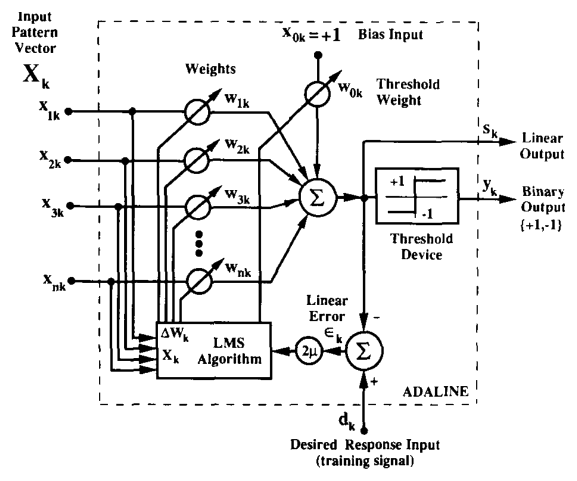
\includegraphics[width=\textwidth,height=0.65\textheight,keepaspectratio]{figuras/paper_adaline.png}\\
  {\scriptsize Fig.~2 del artículo (original) sobre la reconstrucción.}
\end{center}
\column{0.40\textwidth}
\begin{block}{Ecuaciones}
Combinador lineal (producto interno):
\[ s_k = X_k^{T} W_k \]
Cuantizador duro: $y_k = \operatorname{sgn}(s_k) \in \{\pm 1\}$.\\[2pt]
Variante diferenciable: $y_k = \tanh(s_k)$.
\end{block}
\begin{tipbox}
El bias $w_0$ ($+1$) fija el umbral; $s=0$ define el \textbf{hiperplano separador}.
\end{tipbox}
\end{columns}
\end{frame}

\begin{frame}{Separabilidad lineal: el límite del Adaline}
\begin{columns}[T]
\column{0.47\textwidth}
\begin{block}{Un Adaline solo resuelve funciones separables}
Con $n=2$ entradas binarias implementa \textbf{14 de 16} funciones lógicas. Las dos imposibles:
\azul{XOR} y \azul{XNOR}.
\[
\begin{array}{c}
(+1,+1)\to+1 \quad (+1,-1)\to-1\\
(-1,+1)\to-1 \quad (-1,-1)\to+1
\end{array}
\]
\end{block}
\begin{alertblock}{Consecuencia}
No poder realizar \emph{todas} las funciones no es un defecto fatal: \textbf{limita la capacidad y
por eso mejora la generalización}. Para XOR se necesita \azul{no linealidad}.
\end{alertblock}
\column{0.47\textwidth}
\begin{center}
  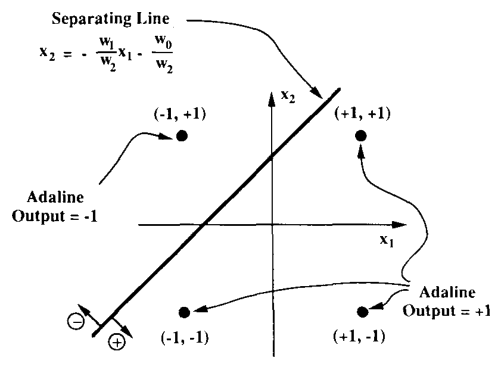
\includegraphics[height=4.6cm, keepaspectratio]{figuras/paper_frontera_lineal.png}\\
  {\scriptsize Fig.~4 del artículo: la condición $s=0$ como \emph{recta separadora} en el espacio de patrones. Ninguna recta separa XOR.}
\end{center}
\end{columns}
\end{frame}

\begin{frame}{Capacidad de patrones: el teorema de Cover}
\begin{columns}[T]
\column{0.47\textwidth}
\begin{center}
  
\includegraphics[width=\textwidth, keepaspectratio]{figuras/fig_cover.png}
\end{center}
\column{0.47\textwidth}
\begin{block}{Probabilidad de separabilidad}
\[
P(N_p,N_w)=2^{1-N_p}\!\sum_{i=0}^{N_w-1}\!\binom{N_p-1}{i} % ,\quad N_p>N_w
\]
\end{block}
\begin{itemize}
  \item Capacidad determinística: $C_d = N_w$ (garantía).
  \item Capacidad estadística: $\azul{C_s \approx 2N_w}$ (promedio).
  \item Baum extendió la cota a redes multicapa.
\end{itemize}
%\begin{ideaclave}
%\emph{Trade-off} capacidad--generalización: entrenar con $N_p \gg N_w/N_y$ para generalizar en vez
%de memorizar.
%\end{ideaclave}
\end{columns}
\end{frame}

\subsection{Clasificadores no lineales}
\begin{frame}{Clasificadores no lineales (I): preprocesador polinomial}
  \begin{itemize}
  \item Con un preprocesador fijo que expande la entrada a términos polinomiales
$[x_1^2,\,x_1,\,x_1x_2,\,x_2,\,x_2^2]$, la condición de umbral $s=0$ se vuelve:
\end{itemize}

\[
s = w_0 + x_1 w_1 + x_1^2 w_{11} + x_1 x_2 w_{12} + x_2^2 w_{22} + x_2 w_2 = 0
\]
\vspace{-10pt}

\begin{itemize}
  \item Frontera \azul{elíptica} $\Rightarrow$ \textbf{resuelve XNOR/XOR} con un solo elemento; los pesos aproximan una \emph{serie de Taylor} (método PDM de Specht, no iterativo).
\end{itemize}
\vspace{-10pt}
\begin{columns}[c]
\column{0.5\textwidth}
\begin{center}
  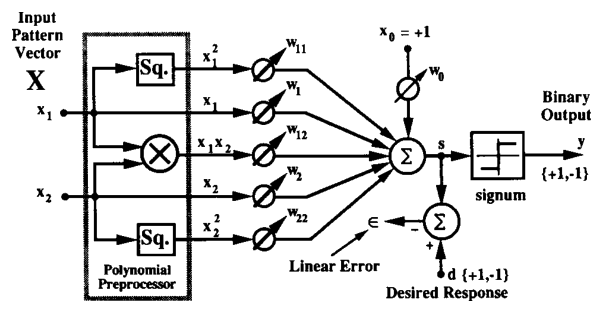
\includegraphics[width=\textwidth,height=0.4\textheight,keepaspectratio]{figuras/paper_preproc_poli.png}\\
  {\scriptsize Fig.~6: Adaline con preprocesador polinomial fijo.}
\end{center}
\column{0.5\textwidth}
\begin{center}
  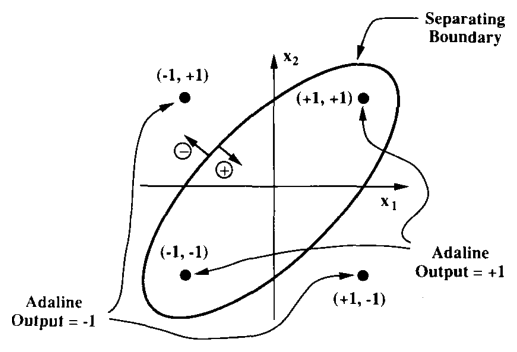
\includegraphics[width=\textwidth,height=0.4\textheight,keepaspectratio]{figuras/paper_elipse_xnor.png}\\
  {\scriptsize Fig.~7: frontera \emph{elíptica} que resuelve XNOR.}
\end{center}
\end{columns}
\end{frame}

% - DIAPOSITIVA EXTRA: Fig.5 curvas de capacidad de Cover -
% (El frame "Capacidad de Cover: las curvas originales" se movió a Experimentos, dividido en E1.)



\begin{frame}{Clasificadores no lineales (II): Madaline I y redes feedforward}
\begin{columns}[T]
\column{0.5\textwidth}
\begin{block}{Madaline I (MRI)}
\begin{itemize}
  \item Capa de Adalines (\emph{signum}) $\to$ \azul{lógica fija} de salida (AND, OR o mayoría).
  \item Primera red en capas entrenable.
  \item \emph{Load-sharing}: ``asignar la responsabilidad a quien pueda asumirla más fácilmente''.
\end{itemize}
\end{block}
\column{0.45\textwidth}
\begin{block}{Red feedforward}
\begin{itemize}
  \item \textbf{Todas} las capas son adaptativas.
  \item Salida: error directo y fácil de adaptar.
  \item \alert{Dificultad clave}: obtener \azul{señales de error} para las capas \textbf{ocultas}.
\end{itemize}
\end{block}
\end{columns}
\begin{ideaclave}
\emph{Backpropagation} y \emph{Madaline Rule III} son precisamente los dos mecanismos que resuelven
el problema de las señales de error en capas ocultas.
\end{ideaclave}
\end{frame}

% - DIAPOSITIVA EXTRA: arquitecturas originales Madaline I y red 3 capas -
\begin{frame}{Las arquitecturas originales: de Madaline~I a la red multicapa }
\vspace{-10pt}
  \begin{columns}[T]
\column{0.5\textwidth}
\begin{center}
  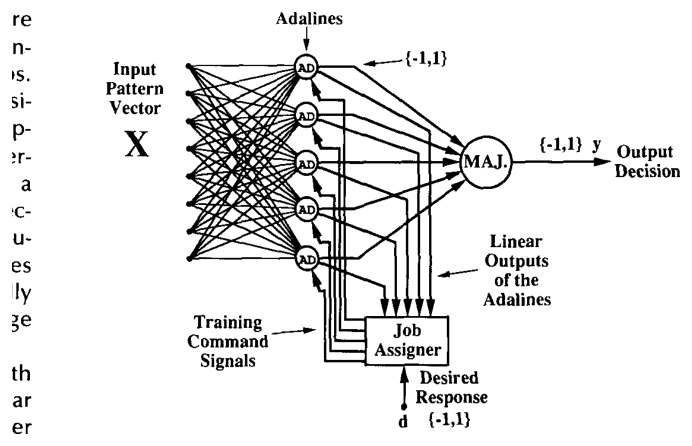
\includegraphics[width=\textwidth,height=0.50\textheight,keepaspectratio]{figuras/paper_madaline1.png}\\
  {\scriptsize Fig.~15: Madaline~I - Adalines \emph{signum} + \azul{lógica fija} .}%(mayoría).}
\end{center}
\begin{tipbox}
El ``\emph{job assigner}'' reparte la responsabilidad usando la salida lineal.
\end{tipbox}
\column{0.5\textwidth}
\begin{center}
  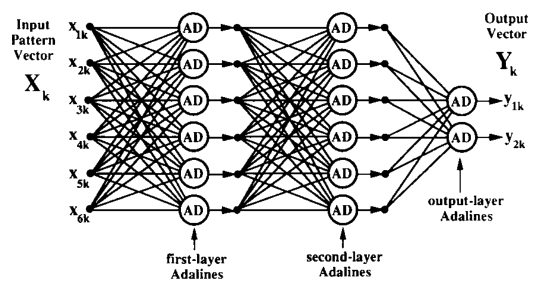
\includegraphics[width=\textwidth,height=0.45\textheight,keepaspectratio]{figuras/paper_red_3capas.png}\\
  {\scriptsize Fig.~11: red \emph{feedforward} de tres capas totalmente conectada.}
\end{center}
\begin{alertblock}{El salto conceptual}
En Madaline~I solo la \textbf{primera} capa es adaptativa; en la red moderna, \azul{todas}.
\end{alertblock}
\end{columns}
\end{frame}

% =====================================================================
\section{Reglas de aprendizaje}
% =====================================================================

\subsection{Corrección de error}
\begin{frame}{Dos familias de reglas y su taxonomía}
\begin{columns}[T]
\column{0.4\textwidth}
\begin{block}{Corrección de error}
Corrigen una \azul{proporción del error} en la respuesta al patrón presente.
\end{block}
\begin{block}{Descenso más pronunciado}
Minimizan el \azul{MSE promediado} sobre todo el conjunto, por gradiente.
\end{block}
\column{0.58\textwidth}
\begin{center}
\resizebox{\textwidth}{!}{%
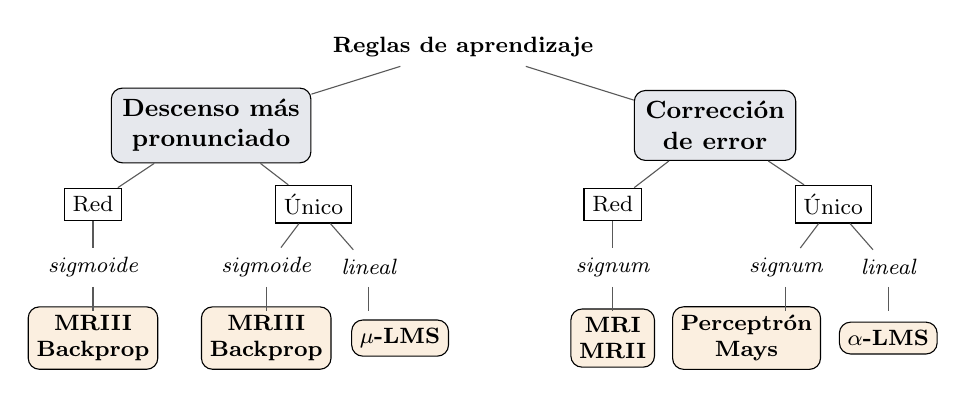
\begin{tikzpicture}[every node/.style={font=\footnotesize}]
  \node (root) at (0,4.2) {\textbf{Reglas de aprendizaje}};
  \node[cat] (sd) at (-3.2,3.2) {Descenso más\\pronunciado};
  \node[cat] (ec) at (3.2,3.2) {Corrección\\de error};
  \draw[ln] (root)--(sd); \draw[ln] (root)--(ec);
  \node[arch] (sdL) at (-4.7,2.2) {Red};
  \node[arch] (sdS) at (-1.9,2.2) {Único};
  \node[arch] (ecL) at (1.9,2.2) {Red};
  \node[arch] (ecS) at (4.7,2.2) {Único};
  \draw[ln] (sd)--(sdL);\draw[ln] (sd)--(sdS);\draw[ln] (ec)--(ecL);\draw[ln] (ec)--(ecS);
  \node[act] (a1) at (-4.7,1.4) {sigmoide};
  \node[act] (a2) at (-2.5,1.4) {sigmoide};
  \node[act] (a3) at (-1.2,1.4) {lineal};
  \node[act] (a4) at (1.9,1.4) {signum};
  \node[act] (a5) at (4.1,1.4) {signum};
  \node[act] (a6) at (5.4,1.4) {lineal};
  \draw[ln] (sdL)--(a1);\draw[ln] (sdS)--(a2);\draw[ln] (sdS)--(a3);
  \draw[ln] (ecL)--(a4);\draw[ln] (ecS)--(a5);\draw[ln] (ecS)--(a6);
  \node[alg] at (-4.7,0.5) {MRIII\\Backprop};
  \node[alg] at (-2.5,0.5) {MRIII\\Backprop};
  \node[alg] at (-0.8,0.5) {$\mu$-LMS};
  \node[alg] at (1.9,0.5) {MRI\\MRII};
  \node[alg] at (3.6,0.5) {Perceptr\'on\\Mays};
  \node[alg] at (5.4,0.5) {$\alpha$-LMS};
  \foreach \x in {-4.7,-2.5,-1.2,1.9,4.1,5.4}{\draw[ln] (\x,1.15)--(\x,0.85);}
\end{tikzpicture}}

{\scriptsize Reproducción fiel de la Fig.~33 del artículo.}
\end{center}
\end{columns}
\end{frame}

\begin{frame}{Corrección de error lineal: $\alpha$-LMS}
\begin{block}{Regla delta de Widrow-Hoff (única regla lineal de corrección)}
\[
W_{k+1} = W_k + \alpha\,\frac{\varepsilon_k}{\lVert X_k\rVert^{2}}\,X_k,
\qquad \varepsilon_k = d_k - X_k^{T} W_k
\]
\end{block}
\begin{columns}[T]
\column{0.5\textwidth}
\begin{itemize}
  \item Corrección proporcional al \azul{error lineal} $\varepsilon_k$.
  \item $\Delta W_k$ colineal con $X_k$ (mínima perturbación).
  \item \naranja{Auto-normalizante}: $\alpha$ no depende de la magnitud de las entradas.
\end{itemize}
\column{0.5\textwidth}
\begin{tipbox}
Estabilidad $0<\alpha<2$; rango práctico $0.1<\alpha<1.0$. El cambio en el error es
$\Delta\varepsilon_k = -\alpha\,\varepsilon_k$.
\end{tipbox}
\end{columns}
\end{frame}

\begin{frame}{Corrección de error no lineal: regla del Perceptrón}
\begin{block}{Rosenblatt}
\[
W_{k+1} = W_k + \alpha\,\frac{\tilde{\varepsilon}_k}{2}\,X_k,
\qquad \tilde{\varepsilon}_k = d_k - y_k \in \{-2,0,+2\}
\]
\end{block}
\begin{columns}[T]
\column{0.54\textwidth}
\begin{itemize}
  \item Usa el \azul{error del cuantizador} $\tilde{\varepsilon}_k$; \textbf{solo adapta si $y_k\neq d_k$}.
  \item \naranja{Teorema de convergencia}: separa en pasos finitos \textbf{si los datos son linealmente separables}.
  \item Si \textbf{no} lo son, el vector de pesos ``gravita hacia cero'' y el algoritmo continúa indefinidamente.
\end{itemize}
\column{0.46\textwidth}
\vspace{-10pt}
\begin{center}
  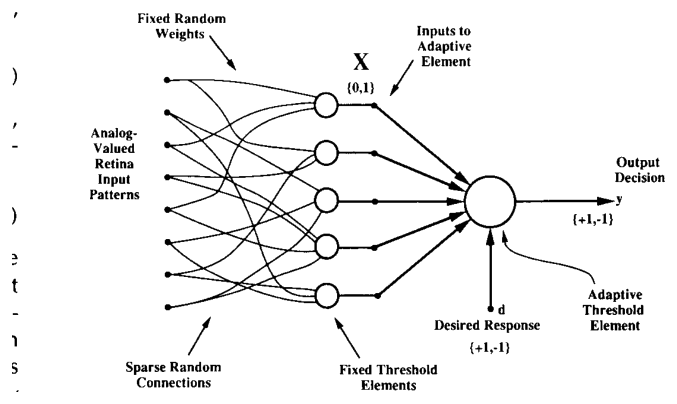
\includegraphics[width=\textwidth,height=0.58\textheight,keepaspectratio]{figuras/paper_perceptron_rosenblatt.png}\\
  {\scriptsize Fig.~13: el $\alpha$-Perceptrón de Rosenblatt - primera capa fija aleatoria + un elemento adaptativo.}
\end{center}
\end{columns}
\end{frame}

\begin{frame}{$\alpha$-LMS \textit{vs.} Perceptrón}
\renewcommand{\arraystretch}{1.25}
\begin{center}
\begin{tabular}{@{}p{0.46\textwidth}|p{0.46\textwidth}@{}}
\toprule
\azul{\textbf{$\alpha$-LMS}} & \azul{\textbf{Perceptrón}} \\
\midrule
$\alpha$ controla estabilidad y convergencia & $\alpha$ solo afecta el tiempo si $W_0\neq0$ \\
Respuestas binarias \textbf{y} continuas & Solo respuestas binarias \\
Puede \textbf{fallar} en separar un conjunto separable & Separa \textbf{cualquier} conjunto separable \\
No da soluciones absurdas con datos no separables & No converge con datos no separables \\
\bottomrule
\end{tabular}
\end{center}
\begin{tipbox}
Objetivos distintos: $\alpha$-LMS reduce el \emph{error lineal}; el Perceptrón busca \emph{separar}.
\end{tipbox}
\end{frame}

\begin{frame}{Reglas de Mays: la ``zona muerta''}
\begin{block}{Adaptación por incremento con zona muerta $\gamma$}
\[
W_{k+1} =
\begin{cases}
W_k + \alpha\,\tilde{\varepsilon}_k\,\dfrac{X_k}{2\lVert X_k\rVert^{2}} & |s_k| \geq \gamma \\[8pt]
W_k + \alpha\,d_k\,\dfrac{X_k}{\lVert X_k\rVert^{2}} & |s_k| < \gamma
\end{cases}
\]
\end{block}
\begin{itemize}
  \item Si es separable: converge en pasos finitos (como el Perceptrón).
  \item Si \textbf{no} lo es: una zona muerta grande \azul{aleja el vector de pesos de cero} $\Rightarrow$ \textbf{mejor que el Perceptrón}.
  \item Casos límite: $\gamma\to0$ recupera el Perceptrón; $\gamma\to\infty$ (relajación) recupera $\alpha$-LMS.
\end{itemize}
\end{frame}

\begin{frame}{Redes multicapa por corrección de error: Madaline Rule II}
\begin{block}{MRII (Widrow, Winter \& Baxter, 1987) - adapta \emph{todas} las capas}
Para cada patrón erróneo:
\begin{enumerate}
  \item Ordenar las Adalines por $|s|$ creciente (mínima perturbación).
  \item \azul{Flip tentativo} de la salida de una Adalina; si reduce el \textbf{error de Hamming}, se acepta.
  \item Reforzar con corrección colineal por $\alpha$-LMS; si no, probar \emph{pares} de Adalines.
  \item Entrenar la capa de salida con $\alpha$-LMS.
\end{enumerate}
\end{block}
\begin{alertblock}{Limitación}
MRII puede \textbf{estancarse en óptimos locales}. Remedio del artículo: \azul{ruido esporádico} en
los pesos o reentrenar con distintas semillas (\emph{random restarts}).
\end{alertblock}
\end{frame}

% - DIAPOSITIVA EXTRA: arquitectura MRII (Fig.16) -
\begin{frame}{La arquitectura Madaline~II del artículo (Fig.~16)}
\vfill
\begin{center}
  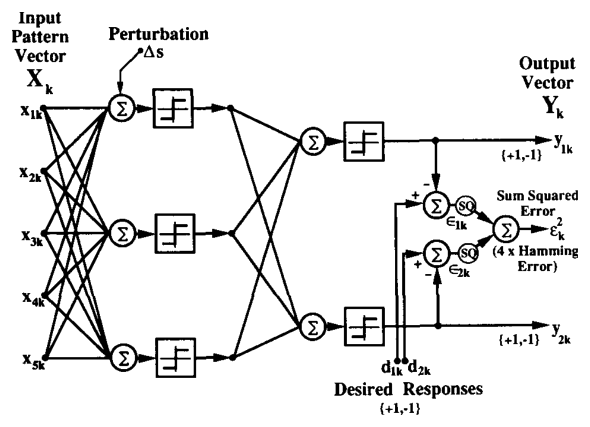
\includegraphics[width=\textwidth,height=0.66\textheight,keepaspectratio]{figuras/paper_mrii.png}
\end{center}
\vfill
{\footnotesize
Red MRII de dos capas, \textbf{ambas adaptativas}. La perturbación $\Delta s$ inyectada en el sumidero
de cada Adalina prueba el \emph{flip} de su salida; si reduce el \azul{error de Hamming} a la salida,
el cambio se refuerza con $\alpha$-LMS.}
\vfill
\end{frame}

\subsection{Descenso de gradiente}
\begin{frame}{Descenso más pronunciado lineal: $\mu$-LMS y la superficie de MSE}
\begin{columns}[T]
\column{0.52\textwidth}
\begin{block}{Regla $\mu$-LMS}
\[ W_{k+1} = W_k + 2\mu\,\varepsilon_k\,X_k \]
Superficie de MSE (paraboloide \azul{convexo}):
\[ \xi(W)=\mathbb{E}[d^2]-2P^{T}W+W^{T}RW \]
Mínimo único: solución de Wiener
\[ W^{*}=R^{-1}P \]
\end{block}
\column{0.46\textwidth}
\begin{itemize}
  \item Gradiente instantáneo $-2\varepsilon_k X_k$: estimador \azul{insesgado} del verdadero.
  \item Estabilidad: $0<\mu<1/\operatorname{tr}[R]$.
  \item Frente a $\alpha$-LMS: $\mu$-LMS converge al \textbf{mínimo MSE} (Wiener); $\alpha$-LMS, a una solución sesgada.
\end{itemize}
\end{columns}
\end{frame}

\begin{frame}{Por qué el gradiente exige activaciones diferenciables}
\begin{center}
  
\includegraphics[width=0.96\textwidth, keepaspectratio]{figuras/fig_superficies_mse.png}
\end{center}
\footnotesize
\vspace{-4pt}
\begin{columns}[T]
\column{0.32\textwidth}
\begin{tipbox}
\textbf{Lineal}: paraboloide convexo, mínimo global garantizado.
\end{tipbox}
\column{0.32\textwidth}
\begin{tipbox}
\textbf{Sigmoide}: suave y navegable; posibles mínimos locales.
\end{tipbox}
\column{0.32\textwidth}
\begin{alertblock}{Signum}
Escalonado, con \textbf{mesetas} de gradiente nulo: el descenso se detiene.
\end{alertblock}
\end{columns}
\end{frame}

% - DIAPOSITIVA EXTRA: superficies MSE originales del artículo (Figs 22-24) -
\begin{frame}{Las superficies de error originales (Figs.~22--24)}
\begin{columns}[T]
\column{0.34\textwidth}
\begin{center}
  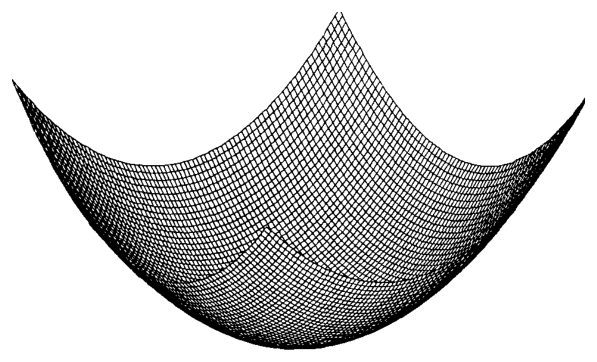
\includegraphics[width=\textwidth,height=0.58\textheight,keepaspectratio]{figuras/paper_mse_lineal.png}\\
  {\scriptsize Fig.~22: error \azul{lineal}.}
\end{center}
\column{0.34\textwidth}
\begin{center}
  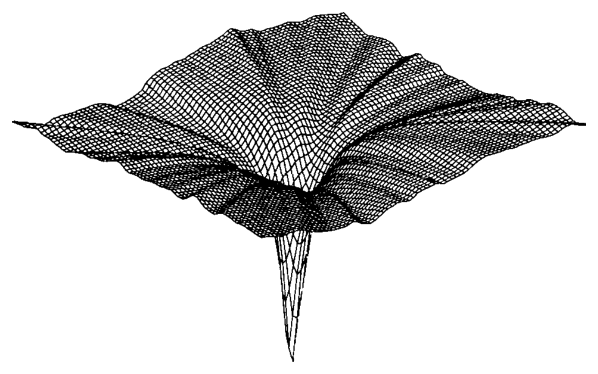
\includegraphics[width=\textwidth,height=0.58\textheight,keepaspectratio]{figuras/paper_mse_sigmoid.png}\\
  {\scriptsize Fig.~23: error \azul{sigmoide}.}
\end{center}
\column{0.34\textwidth}
\begin{center}
  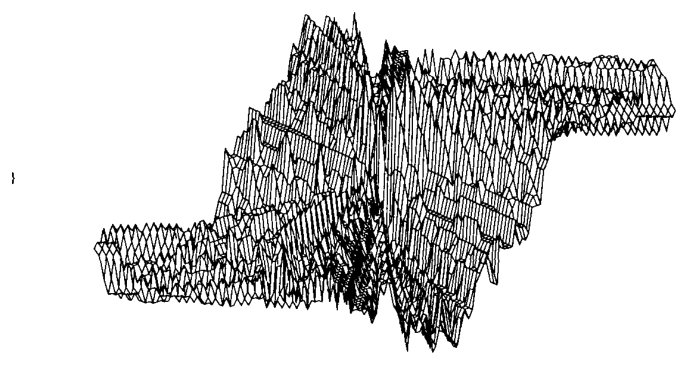
\includegraphics[width=\textwidth,height=0.58\textheight,keepaspectratio]{figuras/paper_mse_signum.png}\\
  {\scriptsize Fig.~24: error \azul{signum}.}
\end{center}
\end{columns}
\vspace{2pt}
\begin{ideaclave}
Las tres provienen del \textbf{mismo} Adaline de dos pesos: el paraboloide liso (lineal) se degrada a
un tazón con mínimos locales (sigmoide) y a un relieve \textbf{escalonado} intratable por gradiente
(signum). Por eso backprop y MRIII usan sigmoides.
\end{ideaclave}
\end{frame}

\begin{frame}{Descenso más pronunciado no lineal: Backpropagation}
\begin{block}{Propagación del error hacia atrás}
Salida (Eq.~79) y capas ocultas (Eq.~87):
\[
\delta^{(L)}_j = \varepsilon_j\,(1-y_j^{2}),
\qquad
\delta^{(l)} = \big(W^{(l+1)T}\delta^{(l+1)}\big)\odot\big(1-(y^{(l)})^{2}\big)
\]
Actualización con \azul{momentum}:
\[
\Delta W_k = \eta\,\Delta W_{k-1} + (1-\eta)\,2\mu\,\delta_k X_k^{T},\qquad \eta\approx 0.8\text{--}0.9
\]
\end{block}
\begin{ideaclave}
$\delta$ \textbf{no es un error}: es una \emph{señal de gradiente} que indica cómo mover cada peso
para reducir el error cuadrático de salida $\varepsilon^2$.
\end{ideaclave}
\end{frame}

% - DIAPOSITIVA EXTRA: arquitectura backprop completa (Fig.25) -
\begin{frame}{La arquitectura de backpropagation del artículo (Fig.~25)}
\vfill
\begin{center}
  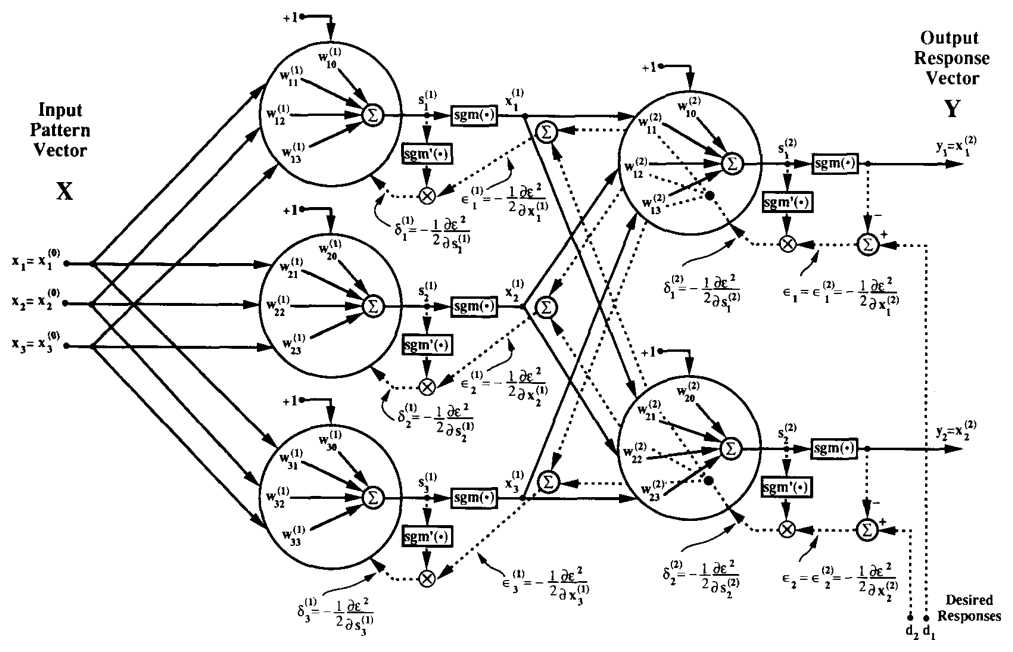
\includegraphics[width=\textwidth,height=0.72\textheight,keepaspectratio]{figuras/paper_bp_red.png}
\end{center}
\vfill
{\footnotesize
Trazo \textbf{continuo} = barrido \azul{hacia adelante} ($X\to Y$); trazo \textbf{punteado} =
barrido \azul{hacia atrás} que transporta los $\delta$. El barrido de retorno tiene la
\textbf{misma complejidad} que el de ida (sin multiplicaciones de peso en la primera capa).}
\vfill
\end{frame}

% - DIAPOSITIVA EXTRA: detalle del combinador (Fig.26) -
\begin{frame}{Detalle de una Adalina en backpropagation (Fig.~26)}
\begin{columns}[T]
\column{0.5\textwidth}
\begin{center}
  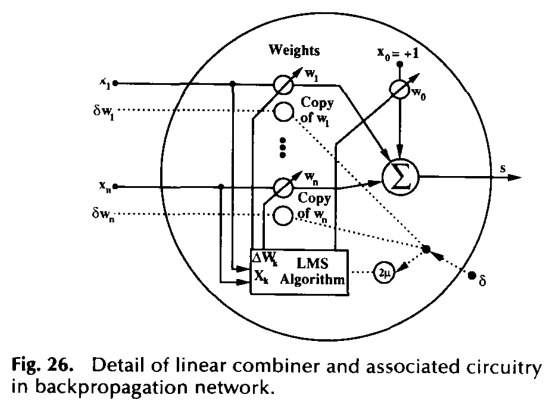
\includegraphics[width=\textwidth,height=0.52\textheight,keepaspectratio]{figuras/paper_bp_detalle.png}\\
  {\scriptsize Fig.~26: combinador con su circuitería de retropropagación y LMS.}
\end{center}
\column{0.5\textwidth}
\begin{block}{Qué muestra el detalle}
\begin{itemize}
  \item Cada Adalina guarda una \azul{copia de sus pesos} para el retorno.
  \item El bloque \textbf{LMS} aplica $\Delta W = 2\mu\,\delta\,X$ al llegar $\delta$.
  \item Los pesos transportan señal en \textbf{ambos sentidos} $\Rightarrow$ difícil en analógico.
\end{itemize}
\end{block}
\begin{ideaclave}
Esa complejidad de doble sentido es la que \textbf{MRIII elimina} usando perturbación.
\end{ideaclave}
\end{columns}
\end{frame}

\begin{frame}{Madaline Rule III $\equiv$ Backpropagation}
\begin{block}{MRIII (Andes, 1988): gradiente por perturbación del sumidero}
Se perturba la suma $s_j$ en $\Delta s$ y se mide el efecto sobre $\varepsilon^2$:
\[
\frac{\partial \varepsilon^2}{\partial s_j} \approx
\frac{\varepsilon^2_{\text{perturbado}} - \varepsilon^2_{\text{base}}}{\Delta s}
\]
\end{block}
\begin{columns}[T]
\column{0.5\textwidth}
\begin{ideaclave}
Cuando $\Delta s \to 0$, MRIII es \textbf{matemáticamente equivalente a backpropagation}.
\end{ideaclave}
\column{0.5\textwidth}
\begin{itemize}
  \item No requiere conocer la derivada de la sigmoide.
  \item \azul{Robusto} para hardware analógico (existió un chip comercial).
  \item Costo: $1+N_{\text{Adalines}}$ pasadas hacia adelante (más caro en digital).
\end{itemize}
\end{columns}
\end{frame}

% - DIAPOSITIVA EXTRA: arquitectura MRIII (Fig.28) vs MRII -
\begin{frame}{MRIII en la red: la misma arquitectura, con sigmoides (Fig.~28)}
\begin{columns}[T]
\column{0.55\textwidth}
\begin{center}
  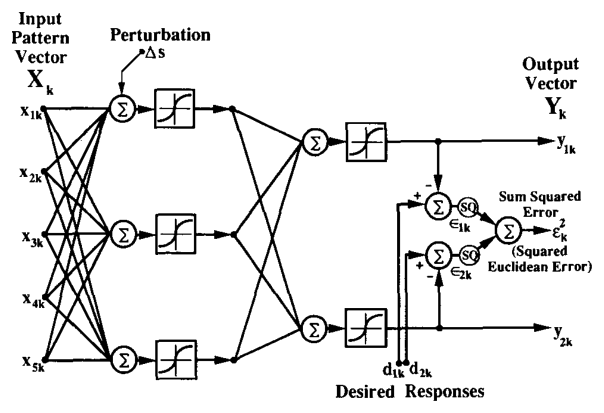
\includegraphics[width=\textwidth,height=0.58\textheight,keepaspectratio]{figuras/paper_mriii_red.png}
\end{center}
\column{0.40\textwidth}
\begin{block}{MRIII $\leftrightarrow$ MRII}
La arquitectura es \textbf{idéntica} a la de MRII (Fig.~16), pero cada cuantizador \emph{signum}
se reemplaza por una \azul{sigmoide}.
\end{block}
\begin{ideaclave}
Ese único cambio hace que el gradiente por perturbación \textbf{coincida con backpropagation},
manteniendo la robustez para hardware analógico.
\end{ideaclave}
\end{columns}
\end{frame}

% =====================================================================
\section{Experimentos}
% =====================================================================

\subsection{Diseño y conjuntos de datos}
% ---------- 1. Contexto + tabla de hipótesis ----------
\begin{frame}{Contexto experimental e hipótesis}

\begin{block}{Objetivo}
El objetivo es \textbf{validar numéricamente} las afirmaciones del artículo: reproducir capacidad,
convergencia, no linealidad y la equivalencia MRIII$\equiv$backprop. Todo se implementó
\azul{desde cero en NumPy} (\emph{scikit-learn} solo para cargar datos y métricas).
\end{block}


\vspace{4pt}
{\footnotesize
\renewcommand{\arraystretch}{1.3}
\begin{tabular}{@{}c p{0.8\textwidth}@{}}
\toprule
\textbf{Hip.} & \textbf{Descripción} \\
\midrule
\azul{H1} & Un Adaline de $N_w$ pesos almacena en promedio $C_s\approx 2N_w$ patrones aleatorios y garantiza $C_d=N_w$ (fórmula de separabilidad de Cover). \\
\azul{H2} & El Perceptr\'on converge en pasos finitos \emph{solo} si los datos son separables (oscila y diverge en norma si no lo son); $\alpha$-LMS y $\mu$-LMS son estables en ambos reg\'imenes, con $\mu$-LMS convergiendo al \'optimo de Wiener $W^*=R^{-1}P$. \\
\azul{H3} & Problemas no separables (XOR) exigen redes multicapa; su entrenamiento cae en óptimos locales y la superficie sigmoide es más navegable que la del signum. \\
\azul{H4} & El gradiente estimado por MRIII (perturbación) coincide numéricamente con el de backpropagation cuando $\Delta s\to 0$. \\
\bottomrule
\end{tabular}}
\end{frame}

% - DIAPOSITIVA EXTRA: detalle de experimentos y datasets -
\begin{frame}{Mapa de experimentos (E1--E7)}
{}
\footnotesize
\renewcommand{\arraystretch}{1.25}
\begin{tabular}{@{}c p{0.3\textwidth} p{0.24\textwidth} p{0.2\textwidth} c@{}}
\toprule
\textbf{Exp.} & \textbf{Problema a evaluar} & \textbf{Algoritmos} & \textbf{Dataset} & \textbf{Hip.} \\
\midrule
E1  & Separabilidad lineal de patrones aleatorios & Programaci\'on Lineal (Monte Carlo) & Binarios aleatorios & \azul{H1} \\
E2  & Fronteras aprendidas \emph{vs.}\ Wiener (separable) & Perceptrón, $\alpha$/$\mu$-LMS & Gaussianos separables & \azul{H2} \\
E3  & Reglas lineales en datos no separables & Perceptr\'on, $\alpha$-LMS, $\mu$-LMS & Gaussianos solapados & \azul{H2} \\
E4  & Superficies de MSE (lineal, sigmoide, signum) & Adaline 2D (sin bias) & 6 patrones aleatorios & --- \\
E5  & Capacidad no lineal (XOR) & MRII \emph{vs.}\ MLP-backprop & XOR ($2^2$) & \azul{H3} \\
E6a & Generalización (flores) & MLP-backprop & Iris & \azul{H3} \\
E6b & Generalización (no lineal 2D) & MLP-backprop & two-moons & \azul{H3} \\
E6c & Clasificación lineal (química) & $\alpha$-LMS, $\mu$-LMS, Wiener & Wine & \azul{H3} \\
E6d & Generalización (dígitos) & MLP-backprop & MNIST-04 & \azul{H3} \\
E7  & Equivalencia de gradientes & MRIII \emph{vs.}\ backprop & Red sigmoide (Iris) & \azul{H4} \\
\bottomrule
\end{tabular}

\vspace{4pt}

%\begin{tipbox}
%Todo implementado \textbf{desde cero en NumPy} ; los conjuntos de datos se
%detallan en las dos láminas siguientes.
%\end{tipbox}


\end{frame}

% - DIAPOSITIVA: datasets sintéticos -
\begin{frame}{Conjuntos de datos sintéticos (E1--E5)}
\begin{center}
  
\includegraphics[width=\textwidth,height=0.4\textheight,keepaspectratio]{figuras/fig_datasets.png}
\end{center}
\begin{columns}[T]
\column{0.52\textwidth}
\begin{block}{Generación controlada}
\begin{itemize}\footnotesize
  \item \azul{Separable}: dos gaussianas alejadas (E2).
  \item \azul{No separable}: gaussianas solapadas (E3).
  \item \azul{XOR}: 4 vértices, exige multicapa (E5).
\end{itemize}
\end{block}
\column{0.48\textwidth}
\begin{tipbox}
Permiten \textbf{conocer la respuesta óptima} (Wiener, Cover) y medir cuánto se le acerca cada regla.
\end{tipbox}
\end{columns}
\end{frame}

% - DIAPOSITIVA: datasets reales con imágenes -
\begin{frame}{Conjuntos de datos reales (E6--E7)}
  \begin{block}{Los cuatro conjuntos reales}
{\footnotesize \azul{Iris} (4 rasgos, 3 clases) \textbullet\ \azul{Wine} (13 rasgos, 3 clases)
\textbullet\ \azul{MNIST-04} (64 rasgos, dígitos 0--4) \textbullet\ \azul{two-moons} (2D no lineal).}
\end{block}
\begin{columns}[T]
\column{0.5\textwidth}
\begin{center}
  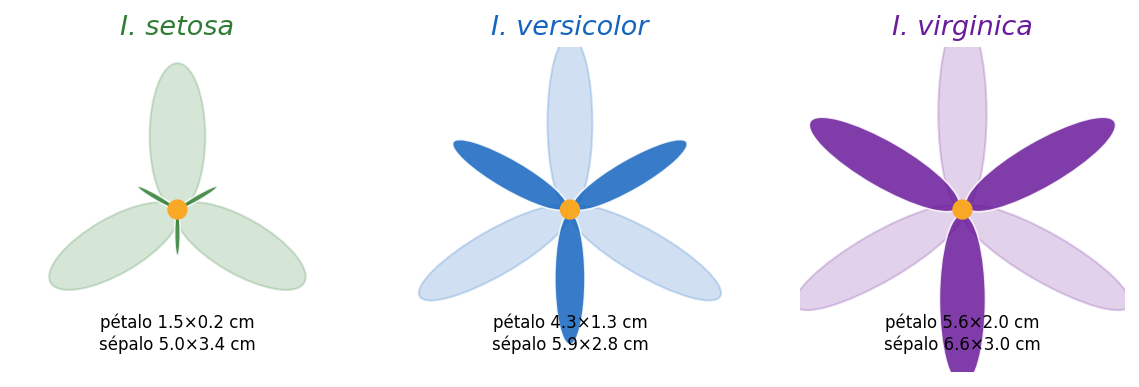
\includegraphics[width=\textwidth,height=0.34\textheight,keepaspectratio]{figuras/fig_iris_clases.png}\\
  {\scriptsize \textbf{Iris} - 3 especies, 4 rasgos (sépalo/pétalo). Esquema con dimensiones reales.}
\end{center}
\column{0.5\textwidth}
\begin{center}
  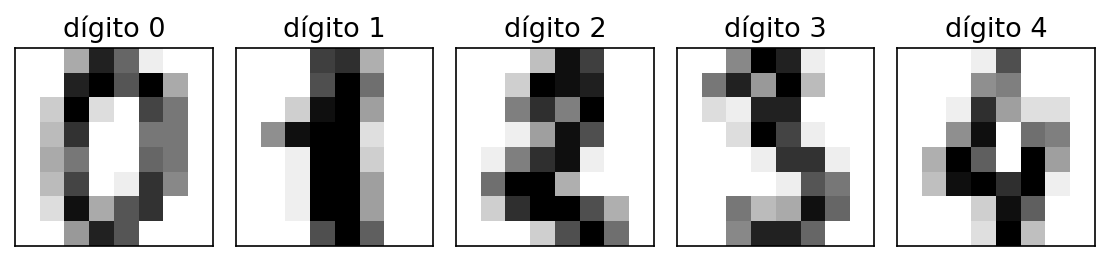
\includegraphics[width=\textwidth,height=0.34\textheight,keepaspectratio]{figuras/fig_mnist04_clases.png}\\
  {\scriptsize \textbf{MNIST-04} - dígitos $0$--$4$, imágenes $8\times8$ (muestras reales).}
\end{center}
\end{columns}
\vspace{2pt}
\end{frame}


\subsection{Resultados}
% ---------- 5. E1 ----------
\begin{frame}{E1 --- Capacidad de Cover}
\begin{columns}[T]
\column{0.5\textwidth}
\begin{center}
  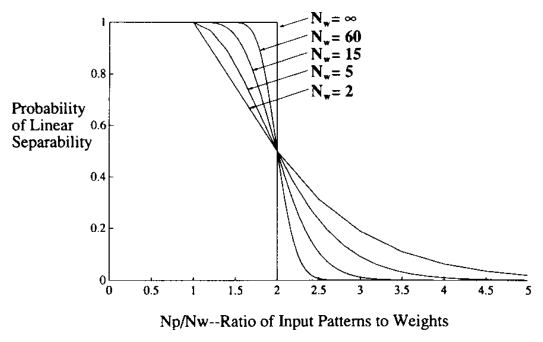
\includegraphics[width=\textwidth,height=0.42\textheight,keepaspectratio]{figuras/paper_cover.png}\\
  {\scriptsize Fig.~5 del artículo (teoría, 1965).}
\end{center}
\column{0.5\textwidth}
\begin{center}
  
\includegraphics[width=\textwidth,height=0.42\textheight,keepaspectratio]{figuras/fig_cover.png}\\
  {\scriptsize Reconstrucción empírica (Monte Carlo).}
\end{center}
\end{columns}
\begin{ideaclave}
\textbf{H1 confirmada}: desviación media $\leq 0.034$ entre empírico y teoría. Se verifica $C_d=N_w$ (en $N_p/N_w=1$) y $C_s\approx 2N_w$ (probabilidad $0.5$).
\end{ideaclave}
\end{frame}

% ---------- 6. E2 ----------
\begin{frame}{E2 --- Reglas lineales \emph{vs.} óptimo de Wiener (separable)}
\begin{center}
  
\includegraphics[width=\textwidth,height=0.5\textheight,keepaspectratio]{figuras/fig_fronteras.png}\\
  {\scriptsize Fronteras aprendidas por cada regla \emph{vs.} la solución de Wiener (datos separables).}
\end{center}
\begin{ideaclave}
\textbf{H2 (parcial) confirmada}: el Perceptrón converge en 2 épocas pero queda a $20.6^\circ$ de Wiener; el $\mu$-LMS a solo $3.5^\circ$ $\Rightarrow$ $\mu$-LMS $\to$ Wiener.
\end{ideaclave}
\end{frame}

% ---------- 7. E3 ----------
\begin{frame}{E3 --- Reglas lineales en datos no separables}
\begin{center}
  
\includegraphics[width=\textwidth,height=0.5\textheight,keepaspectratio]{figuras/fig_noseparable.png}\\
  {\scriptsize Comportamiento de las reglas sobre gaussianos solapados (sin frontera exacta).}
\end{center}
\begin{ideaclave}
\textbf{H2 confirmada}: el Perceptrón \emph{no} converge (oscila); el $\mu$-LMS es el mejor clasificador ($79.6\%$ \emph{vs.} Wiener $81.0\%$) y el de \textbf{menor varianza}.
\end{ideaclave}
\end{frame}

% ---------- 8. E4 ----------
\begin{frame}{E4 --- Superficies de MSE}
\begin{center}
  
\includegraphics[width=0.88\textwidth, keepaspectratio]{figuras/fig_superficies_mse.png}\\
  {\scriptsize Superficies de MSE para un Adaline de 2 pesos (sin bias) sobre 6 patrones aleatorios.}
\end{center}
\vspace{-4pt}
\footnotesize
\begin{columns}[T]
\column{0.32\textwidth}
\begin{tipbox}
\textbf{Lineal} ($\min=0.936$): paraboloide convexo, mínimo global garantizado.
\end{tipbox}
\column{0.32\textwidth}
\begin{tipbox}
\textbf{Sigmoide} ($\min=0.940$): suave y navegable; posibles mínimos locales.
\end{tipbox}
\column{0.32\textwidth}
\begin{alertblock}{Signum ($\min=1.333$)}
Escalonado, con \textbf{mesetas} de gradiente nulo $\Rightarrow$ algoritmos como MRII requieren ruido esporádico.
\end{alertblock}
\end{columns}
\end{frame}

% ---------- 9. E5 ----------
\begin{frame}{E5 --- XOR: MRII \emph{vs.} MLP-Backpropagation}
\begin{columns}[T]
\column{0.58\textwidth}
\begin{center}
  
\includegraphics[width=\textwidth,height=0.55\textheight,keepaspectratio]{figuras/fig_xor.png}\\
  {\scriptsize \textbf{Datos: XOR} (4 patrones, no separable).}
\end{center}
\column{0.42\textwidth}
\renewcommand{\arraystretch}{1.15}
\begin{center}{\scriptsize
\begin{tabular}{@{}lc@{}}
\toprule
Configuración & Éxito \\
\midrule
MRII 2-2-1 & 0/20 \\
MRII 2-3-1 + ruido & 0/20 \\
MLP-BP 2-2-1 & 6/20 \\
MLP-BP 2-3-1 & 11/20 \\
\bottomrule
\end{tabular}}\end{center}
\begin{alertblock}{H3 confirmada}
Solo multicapa resuelve XOR; MRII y backprop sufren óptimos locales.
\end{alertblock}
\end{columns}
\end{frame}

% ---------- 10. E6a Iris ----------
\begin{frame}{E6a --- Generalización: Iris}
\begin{center}
  
\includegraphics[width=\textwidth,height=0.5\textheight,keepaspectratio]{figuras/fig_iris_mlp.png}\\
  {\scriptsize MLP 4-8-3 (backpropagation) sobre \textbf{Iris}: fronteras y matriz de confusión.}
\end{center}
\begin{ideaclave}
\textbf{H3 confirmada}: la red multicapa \azul{generaliza} a datos reales con $91.1\%$ en test, separando 3 clases con solapamiento parcial (versicolor/virginica).
\end{ideaclave}
\end{frame}

% ---------- 11. E6b two-moons ----------
\begin{frame}{E6b --- Generalización: two-moons}
\begin{columns}[T]
\column{0.56\textwidth}
\begin{center}
  
\includegraphics[width=\textwidth,height=0.55\textheight,keepaspectratio]{figuras/fig_moons.png}\\
  {\scriptsize Frontera aprendida sobre \textbf{two-moons} (2D, no lineal).}
\end{center}
\column{0.44\textwidth}
\begin{ideaclave}
\textbf{H3 confirmada}: $93.3\%$ en test. El MLP traza una frontera \azul{curva} que un clasificador lineal no puede $\Rightarrow$ evidencia directa del poder de la no linealidad.
\end{ideaclave}
\end{columns}
\end{frame}

% ---------- 12. E6c Wine ----------
\begin{frame}{E6c --- Clasificación lineal: Wine}
\begin{center}
  
\includegraphics[width=\textwidth,height=0.5\textheight,keepaspectratio]{figuras/fig_wine.png}\\
  {\scriptsize Clasificadores lineales ($\alpha$-LMS, $\mu$-LMS, Wiener) sobre \textbf{Wine} (13 rasgos químicos, 3 cultivares).}
\end{center}
\begin{ideaclave}
\textbf{H3 confirmada}: $98.1\%$ en test con clasificadores lineales. La clase 0 es mayoritariamente separable en el espacio de 13 atributos; Wiener y $\mu$-LMS logran el mejor desempeño.
\end{ideaclave}
\end{frame}

% ---------- 13. E6d MNIST ----------
\begin{frame}{E6d --- Generalización: MNIST-04}
\begin{center}
  
\includegraphics[width=\textwidth,height=0.5\textheight,keepaspectratio]{figuras/fig_mnist.png}\\
  {\scriptsize MLP-backpropagation sobre \textbf{MNIST-04} (dígitos $0$--$4$, imágenes $8\times8$).}
\end{center}
\begin{ideaclave}
\textbf{H3 confirmada}: $98.5\%$ en test sobre 5 clases de dígitos $\Rightarrow$ el backprop escala a entradas de mayor dimensión (64 rasgos) sin perder capacidad de generalización.
\end{ideaclave}
\end{frame}

% ---------- 14. E7 ----------
\begin{frame}{E7 --- Equivalencia MRIII $\equiv$ Backpropagation}
\begin{center}
  
\includegraphics[width=\textwidth,height=0.46\textheight,keepaspectratio]{figuras/fig_mriii_bp.png}\\
  {\scriptsize Gradiente estimado por MRIII (perturbación) \emph{vs.} el analítico de backprop, y su costo.}
\end{center}
\begin{ideaclave}
\textbf{H4 confirmada}: el gradiente de MRIII converge al de backprop con error relativo mínimo de $\azul{5.05\times10^{-8}}$; su costo crece como $\mathcal{O}(N_{\text{Adalines}})$.
\end{ideaclave}
\end{frame}

% =====================================================================
\section{Conclusiones}
% =====================================================================

\subsection{Síntesis y vigencia}
\begin{frame}{Conclusiones}
\begin{block}{Aporte del artículo}
\begin{itemize}
  \item \textbf{Unifica 30 años} de algoritmos bajo un principio común: la \azul{mínima perturbación}.
  \item El linaje Perceptrón $\to$ Adaline $\to$ Madaline $\to$ Backprop es una \textbf{progresión lógica}, no una colección arbitraria.
  \item La equivalencia \azul{MRIII $\equiv$ backprop} muestra que un descubrimiento llega por caminos independientes.
\end{itemize}
\end{block}
\begin{alertblock}{Evaluación de hipótesis}
\textbf{H1--H4 confirmadas}. Matiz en H3: MRII resultó más frágil ante óptimos locales que el MLP
(0/20 por semilla única), tal como el propio artículo anticipa.
\end{alertblock}
\end{frame}

%\begin{frame}{Vigencia: por qué sigue importando hoy}
%\begin{columns}[T]
%\column{0.6\textwidth}
%\begin{block}{Los fundamentos siguen vivos}
%\begin{itemize}
%  \item El \azul{SGD} del \emph{deep learning} es $\mu$-LMS generalizado a redes profundas.
%  \item El \azul{momentum} (Eqs.~96--97) sigue en optimizadores como Adam.
%  \item La perturbación de MRIII anticipa la \azul{optimización de orden cero} (cuando no hay gradiente).
%\end{itemize}
%\end{block}
%\column{0.4\textwidth}
%\begin{ideaclave}
%Comprender la \textbf{geometría del aprendizaje} —hiperplano separador, paraboloide de MSE, mesetas
%del signum— es esencial para diseñar y depurar cualquier sistema de ML.
%\end{ideaclave}
%\end{columns}
%\end{frame}

% ─── CIERRE ──────────────────────────────────────────────────────────
\begin{frame}[plain]
\vfill
\begin{center}
{\Huge\bfseries\azul{Gracias}}\\[10pt]
\footnotesize
30 Years of Adaptive Neural Networks: Perceptron, Madaline, and Backpropagation\\
\emph{B.\ Widrow \& M.\ A.\ Lehr}, Proceedings of the IEEE, 78(9), 1990.
\end{center}
\vfill
\end{frame}

\end{document}
